\documentclass[final]{beamer}
%set image/logo options
\def\RightLogoWidth{0.8}
\def\RightLogoPaddingTop{0.25cm}
\def\RightLogoPaddingBottom{0.5cm}
\def\RightLogo{/Users/willbarnes/Documents/Rice/Posters/posters/logos/RiceLogo_TMCMYK300DPI.jpg}
\def\LeftLogoWidth{2.5}
\def\LeftLogoPaddingTop{1cm}
\def\LeftLogoPaddingBottom{0.5cm}
\def\LeftLogo{/Users/willbarnes/Documents/Rice/Posters/posters/logos/shine-logo.png}
\def\GitHubLogoWidth{0.014\paperwidth}
\def\GitHubLogo{/Users/willbarnes/Documents/Rice/Posters/posters/logos/GitHub-Mark-120px-plus.png}
\def\GitHubUser{wtbarnes}
%set theme
\mode<presentation>
{
\usetheme{I6dv_custom}
}
\setbeamertemplate{caption}[numbered]
%Include packages
\usepackage{soul,color,verbatim}
\usepackage{type1cm}
\usepackage{calc}
%\usepackage{times,mathptmx}
\usepackage{amsmath,amsthm, amssymb, latexsym}
\usepackage{empheq}
\usepackage{graphicx}
\usepackage{epstopdf}
\usepackage[numbers]{natbib}
\usepackage{multicol}
\usepackage{subfigure}
\usepackage[english]{babel}
%\usepackage[latin1]{inputenc}
\usepackage{tikz}
\usetikzlibrary{shapes.geometric, arrows, arrows.meta}
%setup beamerposter package
\usepackage[orientation=portrait,size=custom,width=91.44,height=121.92,scale=1.0]{beamer/beamerposter/beamerposter}
%tikz configuration
%Set tikz options
\tikzstyle{box} = [rectangle, rounded corners, text centered, draw=black]
\tikzstyle{ghost} = [rectangle, rounded corners, text centered, draw=white]
\tikzstyle{arrow} = [-{Latex[width=2mm]},thick]
\tikzstyle{every node} = [font=\footnotesize]
%new commands go here
\newcommand{\ang}{\AA~} %alias angstrom
\setbeamerfont{caption}{size=\footnotesize} %make caption size small

%Set author and title
\title[Modeling Nanoflare Trains]{Understanding the Impact of Nanoflare Heating Frequency\\on the Observed Emission Measure Distribution}
\author[Barnes, Cargill, \& Bradshaw]{Will T. Barnes, Peter J. Cargill, \& Stephen J. Bradshaw}
\institute[Rice University]{Department of Physics and Astronomy, Rice University\\
Space and Atmospheric Physics, The Blackett Laboratory, Imperial College London\\
School of Mathematics and Statistics, University of St. Andrews}
\date{11-15 July, 2016}

%start poster
%everything goes in one frame
\begin{document}
\begin{frame}
  %start columns environment to slice up the page horizontally
  \begin{columns}[T]
  \hfill
  %%
  %%first column
  \begin{column}{0.49\linewidth}
    %introduction
    \begin{block}{Introduction}
    \vspace{-1ex}
    \begin{itemize}
      \item Nanoflare model of \citet{parker_nanoflares_1988}: corona heated by impulsive ($\ll\tau_{cool}$), low-energy ($10^{24}$ erg) events produced by twisting, braiding of field lines rooted in the photosphere
      \item ``Smoking gun'' of nanoflare heating is the faint, high-temperature component of the emission measure distribution, $\mathrm{EM}(T)$ \citep{cargill_implications_1994,cargill_nanoflare_2004}
      \item While ``hot'' (i.e. $>10^{6.6}$ K) part of $\mathrm{EM}(T)$ poorly constrained observationally \citep{winebarger_defining_2012}, measurements of the cool ($10^6<T<10^{6.6}$ K) part of $\mathrm{EM}(T)$ in AR cores are consistent with loop models heated by intermediate frequency nanoflares \citep{reep_diagnosing_2013,cargill_active_2014}.
      \item Fundamental question: \alert{what is the frequency of energy release in the solar corona?} Two extreme cases:
      \begin{itemize}
        \item Low-frequency heating: Time between successive events is much greater than typical loop cooling time (i.e. approaches single nanoflare case)
        \item High-frequency heating: Time between successive events is much smaller than typical loop cooling time (i.e. approaches steady heating case)
      \end{itemize}
      \item \textbf{Goal:} \alert{Use hydrodynamic loop models to better understand how different heating properties, including the heating frequency, affect the ``hot'' part of the emission measure distribution.}
    \end{itemize}
    \end{block}
    %hydrodynamics
    \begin{block}{Hydrodynamic Modeling}
      \vspace{-1ex}
      \begin{itemize}
        \item Zero-dimensional Enthalpy-based Thermal Evolution of Loops (EBTEL) model of \citet{klimchuk_highly_2008,cargill_enthalpy-based_2012} allows for efficient modeling of many thousands of loops
        \item We use a modified form of the EBTEL model to treat the electron and ion populations separately \citep[for more details, see][submitted]{barnes_inference_2016}
        \item Applying the ``EBTEL method'' to the two-fluid hydrodynamic equations \citep[as given in][]{bradshaw_influence_2013}, the modified two-fluid EBTEL equations are,
        \begin{align}
          \frac{d}{dt}\bar{p}_e &= \frac{\gamma - 1}{L}\left\lbrack\psi_{TR} - (\mathcal{R}_{TR} + \mathcal{R}_C)\right\rbrack + k_B\bar{n}\nu_{ei}(\bar{T}_i - \bar{T}_e) + (\gamma - 1)\bar{Q}_e,\label{eq:ebtel_pe} \\[0.5em]
		      \frac{d}{dt}\bar{p}_i &= -\frac{\gamma - 1}{L}\psi_{TR} + k_B\bar{n}\nu_{ei}(\bar{T}_e - \bar{T}_i) + (\gamma - 1)\bar{Q}_i,\label{eq:ebtel_pi}\\[0.5em]
		      \frac{d}{dt}\bar{n} &= \frac{c_2(\gamma - 1)}{c_3\gamma Lk_B\bar{T}_e}\left(\psi_{TR} - F_{ce,0} - \mathcal{R}_{TR}\right),\label{eq:ebtel_n}
        \end{align}
        where $c_1=\mathcal{R}_{TR}/\mathcal{R}_C$, $c_2=\bar{T}/T_a=0.9$, $c_3=T_0/T_a=0.6$, $\psi_{TR}$ is a term included to maintain charge and current neutrality, and $\nu_{ei}$ is the electron-ion binary Coulomb collision frequency
        \item Assume quasi-neutrality, $n_e=n_i=n$, and closed by equations of state: $p_e=k_BnT_e$ and $p_i=k_BnT_i$
      \end{itemize}
    \end{block}
    %single-pulse results
    \begin{block}{Single-nanoflare Results}
      \vspace{-1ex}
      \begin{itemize}
        \item Single nanoflare is the most extreme low-frequency case, loop allowed to undergo complete heating and cooling cycle
        \item In \citet[submitted]{barnes_inference_2016}, we investigated the effect of pulse duration ($\tau$), heat flux limiting, electron versus ion heating, and non-equilibrium ionization (NEI) on the resulting emission measure distribution, $\mathrm{EM}(T)$
        \item We found that,
        \begin{itemize}
          \item While very short pulses ($\tau=20,40$ s) lead to significant emission above 10 MK, comparisons with field-aligned models \citep[e.g. HYDRAD,][]{bradshaw_influence_2013} show that EBTEL gives an artifically fast rise in density and thus an excess of hot emission for these very short heating times; longer pulses ($\tau=200,500$ s) show a cutoff near 10 MK.
          \item Compared to pure Spitzer thermal conduction, heat flux limiting (using $f=1/6$) extends $\mathrm{EM}(T)$ to $>10$ MK; extreme values of $f$ (e.g. $f=1/30$) lead to significant emission $>20$ MK.
          \item For the case in which the ions are heated, no emission is visible above 8 MK, independent of the pulse duration
          \item Including effects due to NEI shows that, even for very short pulses, there is little to no emission visible above 10 MK, for the single-fluid, electron heating, and ion heating cases
        \end{itemize}
        \item Conclusion: \alert{$\mathrm{EM}(T)$ signature of loop plasma heated by a single nanoflare is most likely found in the temperature range $T_m<T<10^7$ K}, where the temperature of maximum emission $T_m\approx4$ MK for active region (AR) cores \citep{warren_systematic_2012}
      \end{itemize}
      \vspace{-1ex}
      \begin{figure}
        \subfigure{%
        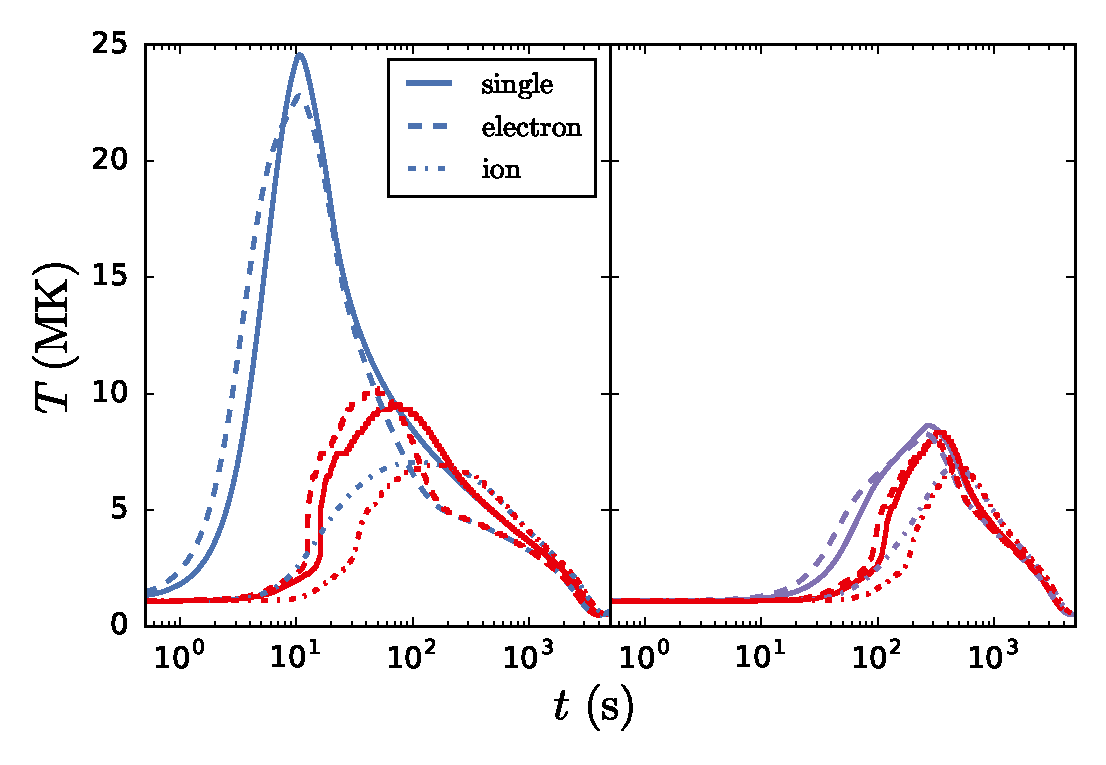
\includegraphics[width=0.49\columnwidth]{figures/single_pulse_Tn_profiles.eps}
        \label{fig:single_Tn_profiles}}
        \subfigure{%
        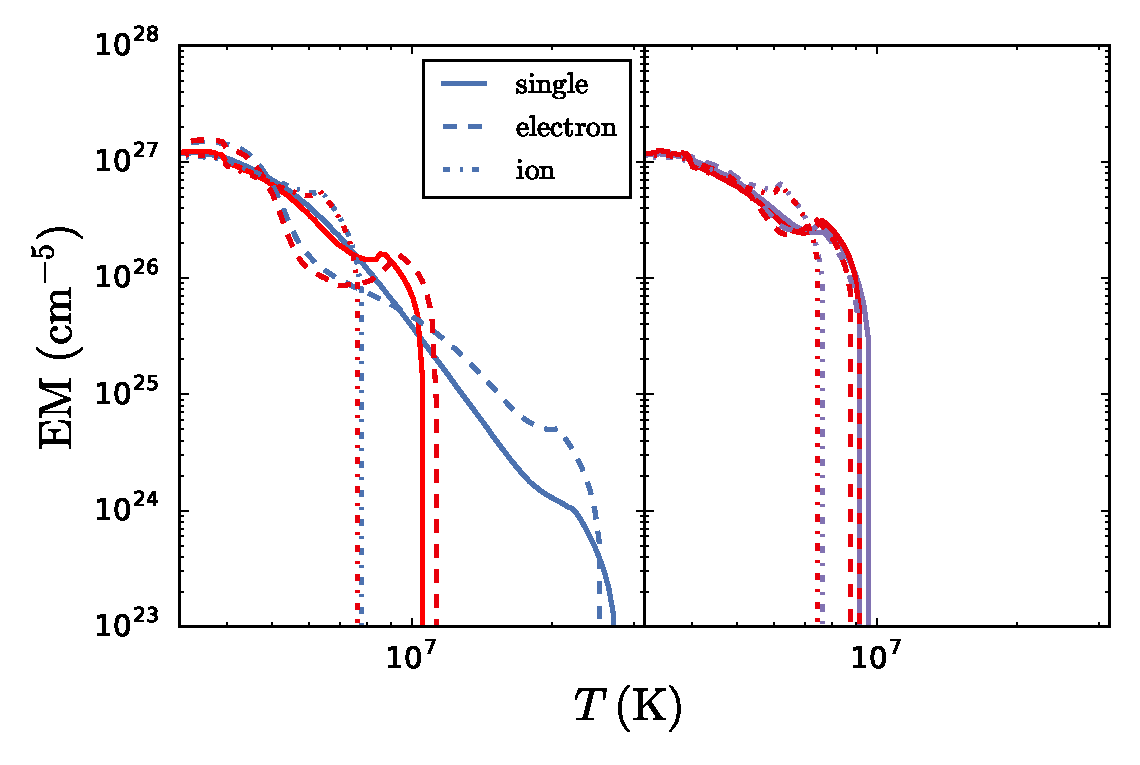
\includegraphics[width=0.49\columnwidth]{figures/single_pulse_em_dist.eps}
        \label{fig:single_em_dist}}
        \caption{Equilibrium and non-equilibrium (red) ionization results for a single nanoflare lasting 20 s (blue) and 500 s (purple) in the single-fluid case (solid) as well as the case in which only the electrons (dashed) or only the ions (dot-dashed) are heated. \textbf{Left:} the electron temperature as a function of time for a 20 s pulse (left) and a 500 s pulse (right). \textbf{Right:} corresponding $\mathrm{EM}(T)$ for the equilibrium (left, blue and right, purple) and NEI (red) cases.}
      \end{figure}
      \vspace{-2ex}
    \end{block}
    %energy budget and heating stats
    \begin{block}{Energy Budget and Heating Statistics}
      \begin{columns}[T]
      \begin{column}{0.49\columnwidth}
        \vspace{-2ex}
        \begin{figure}
          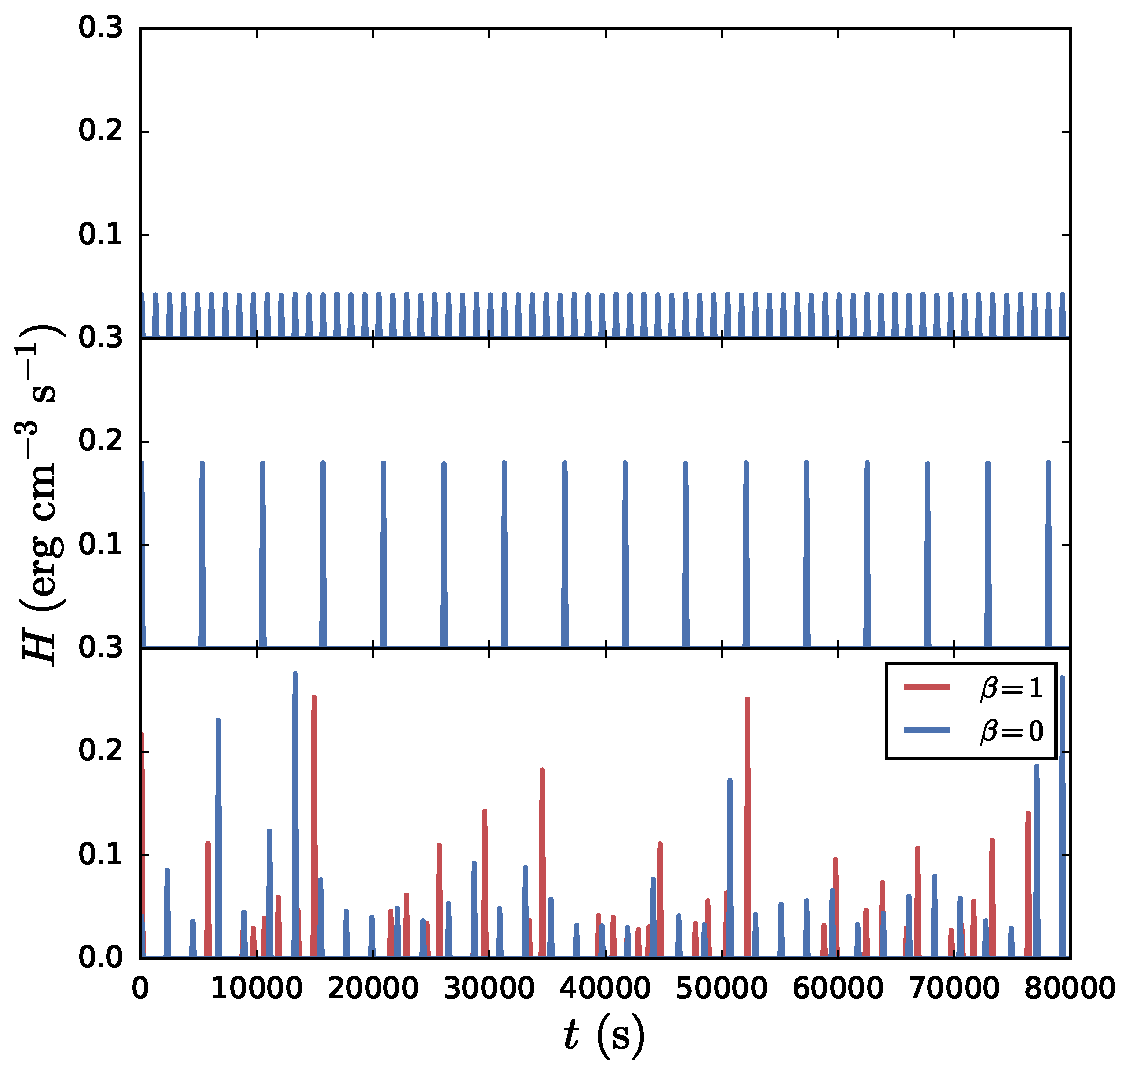
\includegraphics[width=\columnwidth]{figures/heating_functions.pdf}
          \caption{Top (Middle) panel shows Uniform heating amplitudes for $t_N=1000$ ($t_N=5000$) s. Bottom panel shows Heating amplitudes drawn from a power-law distribution with  $\alpha=-1.5$ and mean wait time $t_N=2000$ s; the events shown in red (blue) have wait times that depend on the previous event energy (uniform wait times).}
          \label{fig:heating_funcs}
        \end{figure}
      \end{column}
      \begin{column}{0.49\columnwidth}
        \vspace{-6ex}
        \begin{figure}
          \centering
          	\begin{tikzpicture}[node distance=3.75cm]
		%Draw the nodes
		\node (species) [ghost] {Heated Species $=\left\{
		\begin{array}{l}
			\mathrm{electron} \\
			\mathrm{ion} \\
			\mathrm{single}
		\end{array}
		\right.$};
		\node (ghost_ph) [ghost, below of=species] {};
		\node (alpha_pl) [ghost, left of=ghost_ph] {$\alpha=\left\{
		\begin{array}{l}
			-1.5 \\
			-2.0 \\
			-2.5
		\end{array}
		\right.$};
		\node (alpha_uni) [ghost, right of=ghost_ph] {uniform};
		\node (beta) [ghost, below of=alpha_pl]{$\beta=\left\{
		\begin{array}{l}
			0 \\
			1
		\end{array}
		\right.$};
		%wait time pl
		\begin{scope}[node distance=1.8cm]
		\node (tni_pl) [ghost, below of=beta]{$t_N=t_{N,i}$};
		\node (ell1_pl) [ghost, left of=tni_pl]{$\ldots$};
		\node (tn0_pl) [ghost, left of=ell1_pl]{$t_N=250$ s};
		\node (ell2_pl) [ghost, right of=tni_pl]{$\ldots$};
		\node (tn1_pl) [ghost, right of=ell2_pl]{$t_N=5000$ s};
		%wait time uniform
		\node (tni_uni) [ghost, below of=alpha_uni]{$t_N=t_{N,i}$};
		\node (ell1_uni) [ghost, left of=tni_uni]{$\ldots$};
		\node (tn0_uni) [ghost, left of=ell1_uni]{$t_N=250$ s};
		\node (ell2_uni) [ghost, right of=tni_uni]{$\ldots$};
		\node (tn1_uni) [ghost, right of=ell2_uni]{$t_N=5000$ s};
		\end{scope}
		%number of runs uniform
		\node (nr0) [ghost, below of=tn0_pl]{$N_R=\left\{
		\begin{array}{l}
			1 \\
			2 \\
			\vdots \\
			57
		\end{array}
		\right.$};
		\node (nri) [ghost, below of=tni_pl]{$N_R=\left\{
		\begin{array}{l}
			1 \\
			2 \\
			\vdots \\
			N_{R,i}
		\end{array}
		\right.$};
		\node (nr1) [ghost, below of=tn1_pl]{$N_R=\left\{
		\begin{array}{l}
			1 \\
			2 \\
			\vdots \\
			625
		\end{array}
		\right.$};
		%Draw the arrows
		\draw [arrow] (species) -- (alpha_pl);
		\draw [arrow] (species) -- (alpha_uni);
		\draw [arrow] (alpha_pl) -- (beta);
		\draw [arrow] (beta) -- (tni_pl);
		\draw [arrow] (beta) -- (tn0_pl);
		\draw [arrow] (beta) -- (tn1_pl);
		\draw [arrow] (tni_pl) -- (nri);
		\draw [arrow] (tn0_pl) -- (nr0);
		\draw [arrow] (tn1_pl) -- (nr1);
		\draw [arrow] (alpha_uni) -- (tni_uni);
		\draw [arrow] (alpha_uni) -- (tn0_uni);
		\draw [arrow] (alpha_uni) -- (tn1_uni);
	\end{tikzpicture}

          \caption{Heating function parameter space. We consider a range of waiting times $250<t_N<5000$ s, in increments of 250 s. In the power-law case, a sufficiently large number of runs, $N_R$ is required to sample the distribution. For example, when $t_N=5000$ s, $N_R=625$ such that for each $(\alpha,\beta,t_N=5000)$, we run the model 625 times.}
          \label{fig:parameter_space}
        \end{figure}
        \vspace{-2ex}
      \end{column}
      \end{columns}
      \begin{itemize}
        \item Loop of half-length $L=40$ Mm heated by $N$ triangular pulses with duration $\tau=200$ s over $t_{total}=8\times10^4$ s.
        \item Each event has maximum heating rate $H_i$ and followed by a waiting time of $t_{N,i}$; static background heating $H_{bg}=3.5\times10^{-5}$ erg cm$^{-3}$ s$^{-1}$
        \item $H_i$ can either be uniform such that $H_i=H_0$ for all $i$ or chosen from a power-law distribution with $\alpha=-1.5,-2.0,-2.5$
        \item The total energy injected into the loop is constrained by,
          \begin{equation}
            H_{eq} = \frac{1}{t_{total}}\sum_{i=1}^N\int_{t_i}^{t_i+\tau}\mathrm{d}t~Q(t) = \frac{\tau}{2t_{total}}\sum_{i=1}^NH_i,
          \end{equation}
        \item $H_{eq}\approx3.6\times10^{-3}$ erg cm$^{-3}$ s$^{-1}$ is the time-averaged heating rate such that $T_{m}\approx4$ MK, consistent with AR core observations \citep{warren_systematic_2012}.
        \item Treat $t_{N,i}$ as time needed for the field to ``unwind'', consistent with the \citet{parker_nanoflares_1988} nanoflare picture
        \begin{itemize}
          \item $\beta=0$: $t_{N,i}=t_N$ for all $i$, no dependence on $H_i$
          \item $\beta=1$: $\varepsilon=LA\tau H_i/2\propto t_{N,i}$ (see bottom panel of Fig. \ref{fig:heating_funcs})
        \end{itemize}
        \item Total number of events dependent on $t_N$, $N=t_{total}/(t_N + \tau)$ such that $N=16$ when $t_N=5000$ s
        \item For the power-law cases, require $NN_R\sim1\times10^4$, where $N_R$ is the number of runs for each unique point in the parameter space, $(\alpha,\beta,t_N)$
      \end{itemize}
    \end{block}
  \end{column}
  %%
  %%second column
  \begin{column}{0.49\linewidth}
    %em distribution
    \begin{block}{Emission Measure Distribution}
      \vspace{-1ex}
      \begin{itemize}
        \item Compute solutions to Eqs. \ref{eq:ebtel_pe}, \ref{eq:ebtel_pi}, and \ref{eq:ebtel_n} for all $N_R$ runs for each point in the multidimensional heating parameter space. (Note: for the events of uniform magnitude, $N_R=1$)
        \item To account for NEI, we use the numerical code described in \citet{bradshaw_numerical_2009} to calculate the fractional ionization states for Fe IX through Fe XXVII and calculate $T_{eff}$, a temperature that would be measured based on the actual ionization states
        \item Given a temperature range $4\le\log{T_e}\le8.5$ with bin widths $\Delta\log{T_e}=0.01$, at each time $t_j$, add $n_j^2(2L)$ to every bin that falls in the range $[T_{0e,j},T_{ae,j}]$; time-averaging over the entire run gives $\mathrm{EM}(T)$
        \item To calculate $\mathrm{EM}(T_{eff})$, we use the same procedure, but using $T_{eff}$ instead of $T_e$.
      \end{itemize}
      \vspace{-2ex}
      \begin{figure}
        \centering
        \subfigure{%
        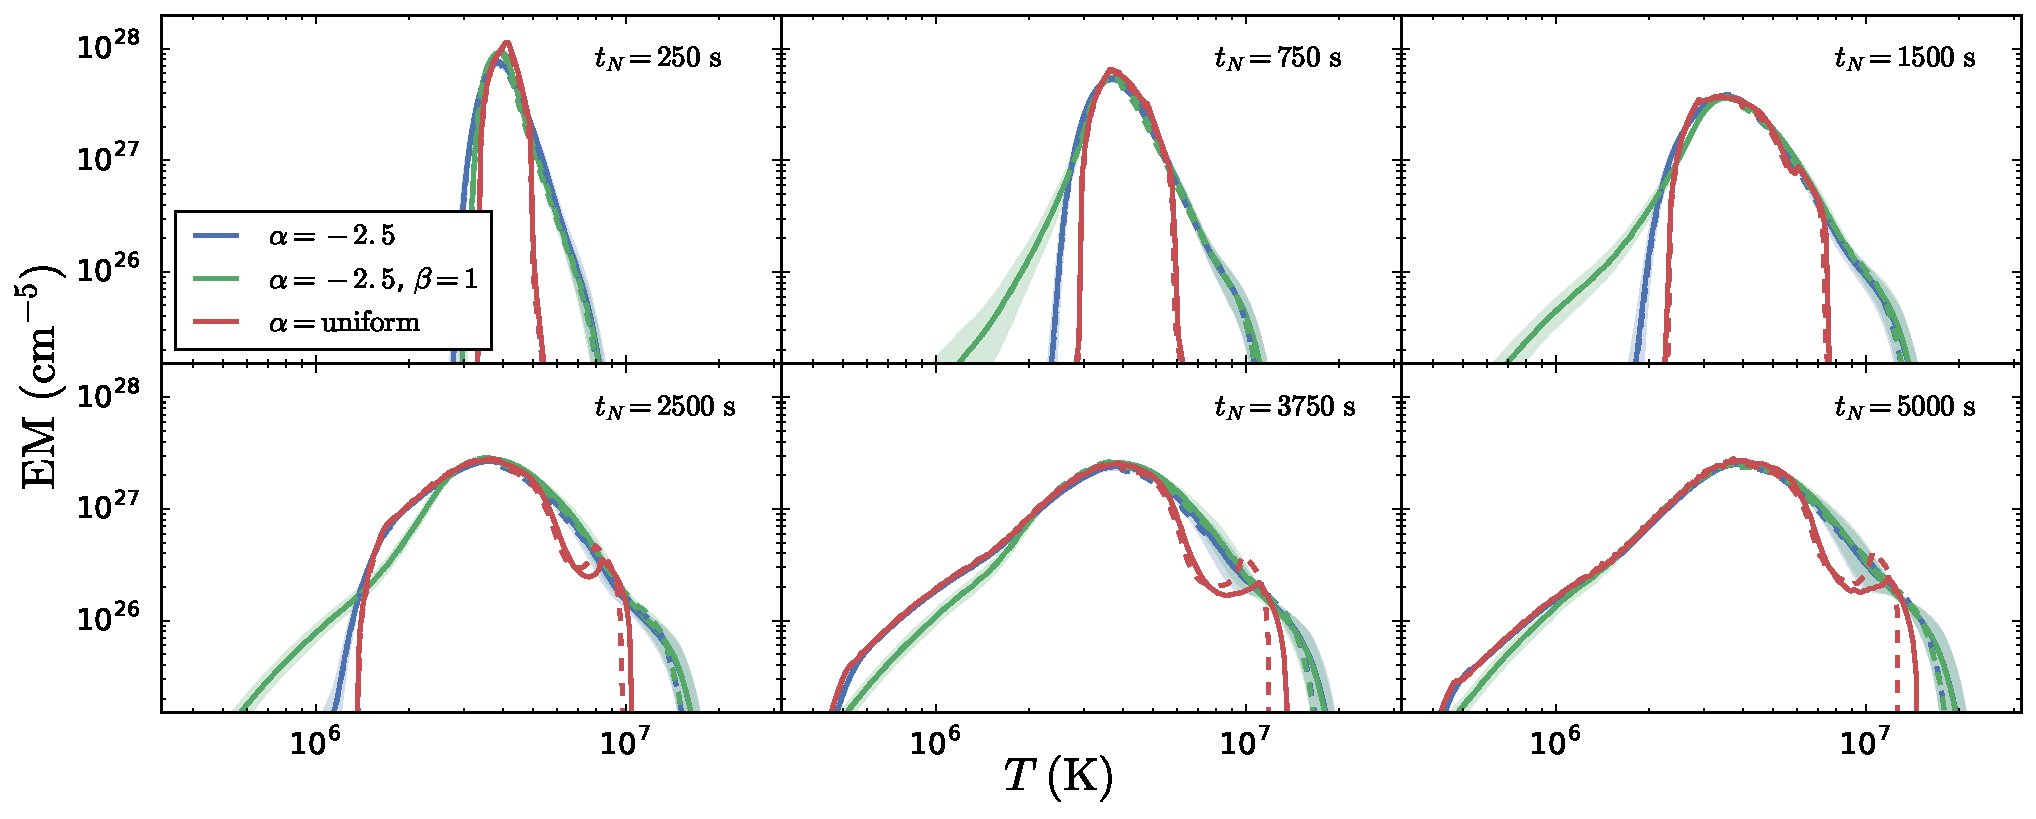
\includegraphics[width=\columnwidth]{figures/em_grid_electron_a25.pdf}
        \label{fig:electron_em}}
        \subfigure{%
        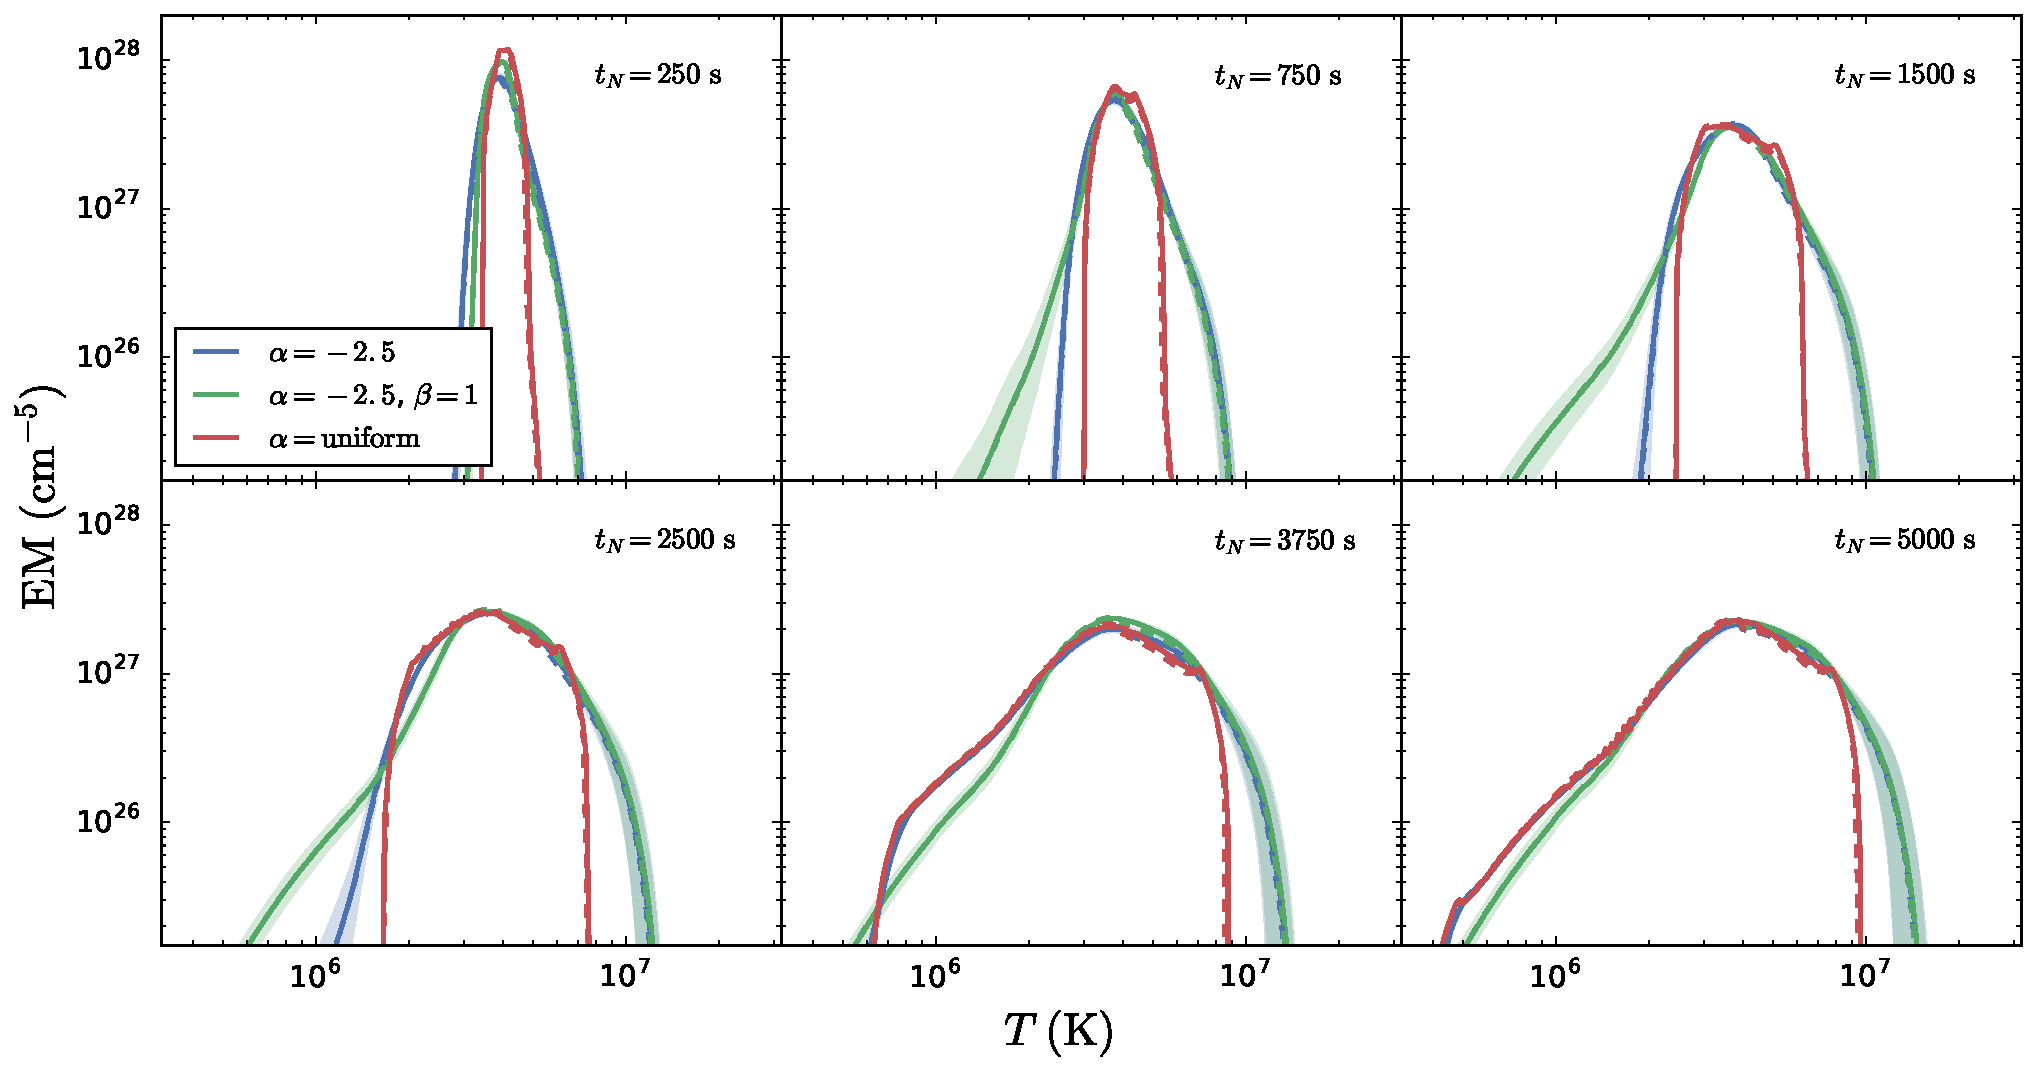
\includegraphics[width=\columnwidth]{figures/em_grid_ion_a25.pdf}
        \label{fig:ion_em}}
        \caption{Emission measure distributions for waiting-times $t_N=250,750,1500,2500,3750,5000$ s in the electron (top) and ion (bottom) heating cases. The three types of heating functions shown are uniform heating rates (red), heating rates chosen from a power-law distribution of $\alpha=-2.5$ (blue), and heating rates chosen from a power-law distribution of $\alpha=-2.5$ where the time between successive events is proportional to the heating rate of the preceding event (green). The solid lines in the two power-law cases show the mean $\mathrm{EM}(T)$ over $N_R$ runs and the shading indicates $1\sigma$ from the mean. The dashed lines denote the corresponding $\mathrm{EM}(T_{eff})$ distribution. The standard deviation is not included in the NEI results.}
      \end{figure}
      \vspace{-2ex}
    \end{block}
    %em ratio
    \begin{block}{Hot Plasma Diagnostics}
      \vspace{-1ex}
      \begin{itemize}
        \item Well-known cool emission measure scaling $\mathrm{EM}(T)\propto T^a$;  similar scaling claimed for the hot part of the emission measure distribution, $\mathrm{EM}(T)\propto T^{-b}$ over a temperature range $T_m\lesssim T\lesssim10^{7.2}$.
        \item Observations have shown $7\lesssim b\lesssim10$ \citep{warren_systematic_2012} though measurements of $b$ are poorly constrained due to lack of spectroscopic data in this temperature range; $b$ very sensitive to the temperature range over which the fit is performed.
        \item \citet{brosius_pervasive_2014} find the ratio of Fe XIX (formed at $T\approx10^{6.95}$ K) to Fe XII (formed at $T\approx10^{6.2}$ K) intensity to be $\sim0.59$ inside AR core compared to $\sim0.076$ outside, providing possible evidence for impulsive heating.
        \item As a proxy for this intensity ratio and an alternative to $b$, we compute an emission measure ratio $\mathrm{EM}(T_{hot})/\mathrm{EM}(T_{cool})$, with $T_{hot}=10^{6.95}$ K and $T_{cool}=10^{6.3}\approx2\times10^6$ K.
      \end{itemize}
      \vspace{-2ex}
      \begin{figure}
        \centering
        \subfigure[Electron heating, grouped by $(\alpha,\beta)$]{%
        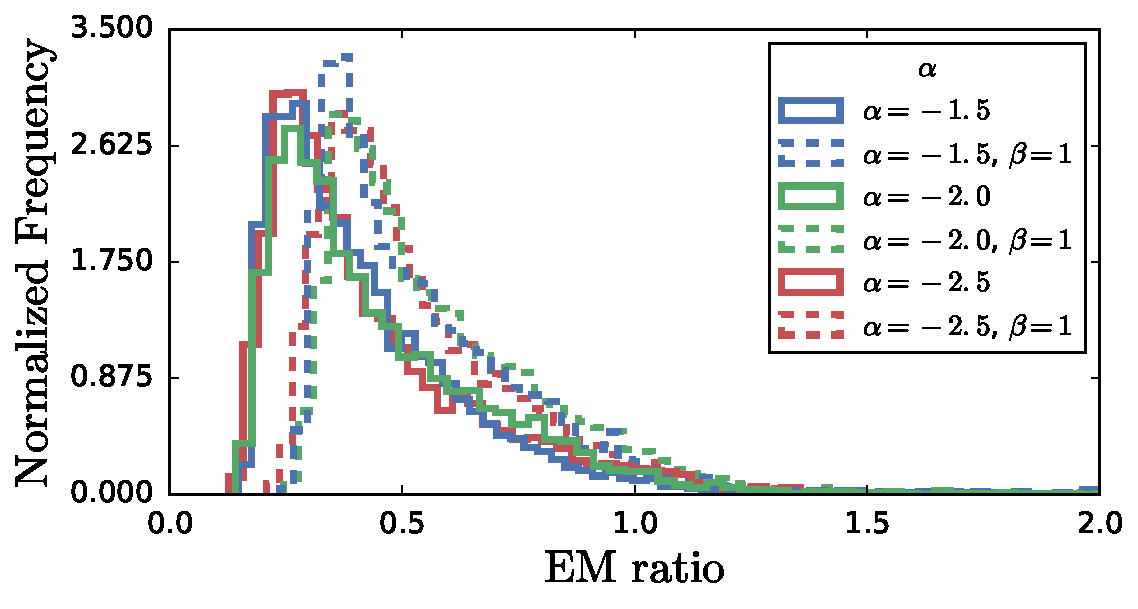
\includegraphics[width=0.49\columnwidth]{figures/ratio_hist_alpha_electron_T2.pdf}
        \label{fig:ratio_electron_alpha}}
        \subfigure[Electron heating, grouped by $t_N$]{%
        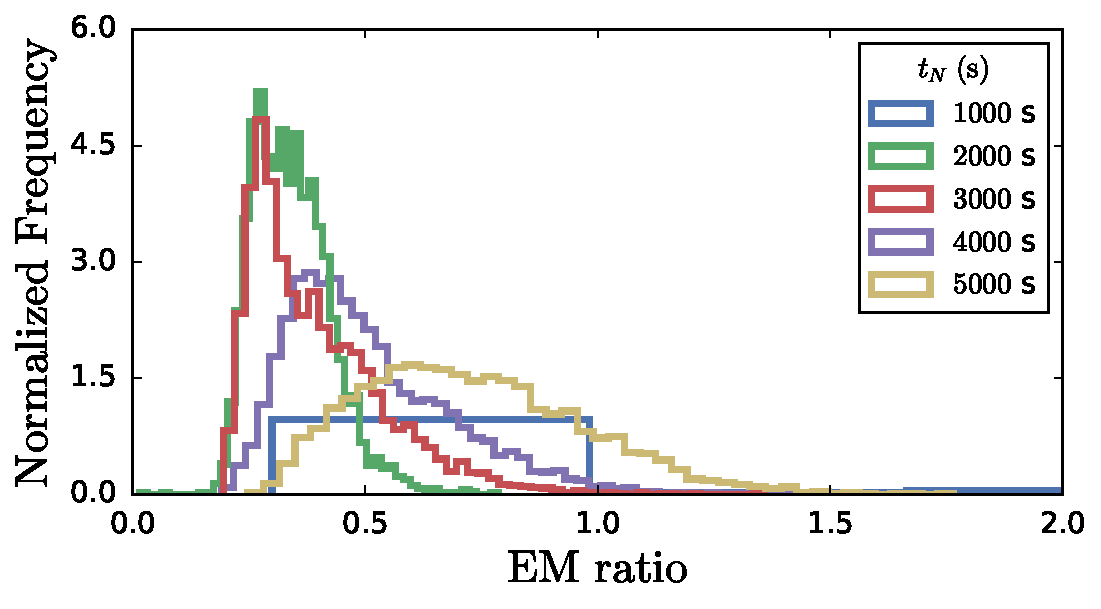
\includegraphics[width=0.49\columnwidth]{figures/ratio_hist_twait_electron_T2.pdf}
        \label{fig:ratio_electron_twait}}
        \subfigure[Ion heating, grouped by $(\alpha,\beta)$]{%
        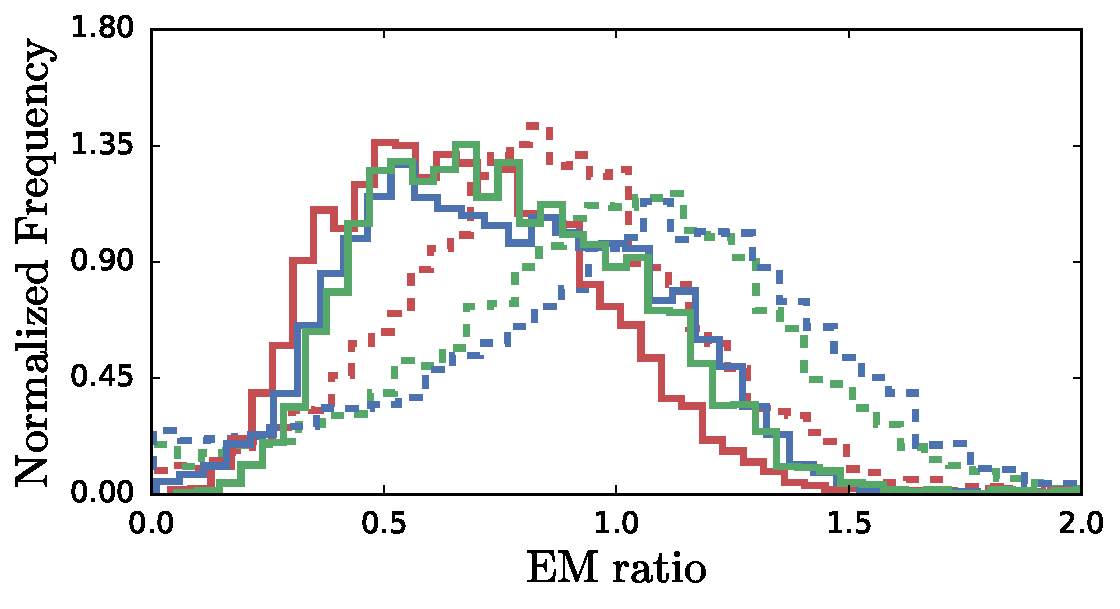
\includegraphics[width=0.49\columnwidth]{figures/ratio_hist_alpha_ion_T2.pdf}
        \label{fig:ratio_ion_alpha}}
        \subfigure[Ion heating, grouped by $t_N$]{%
        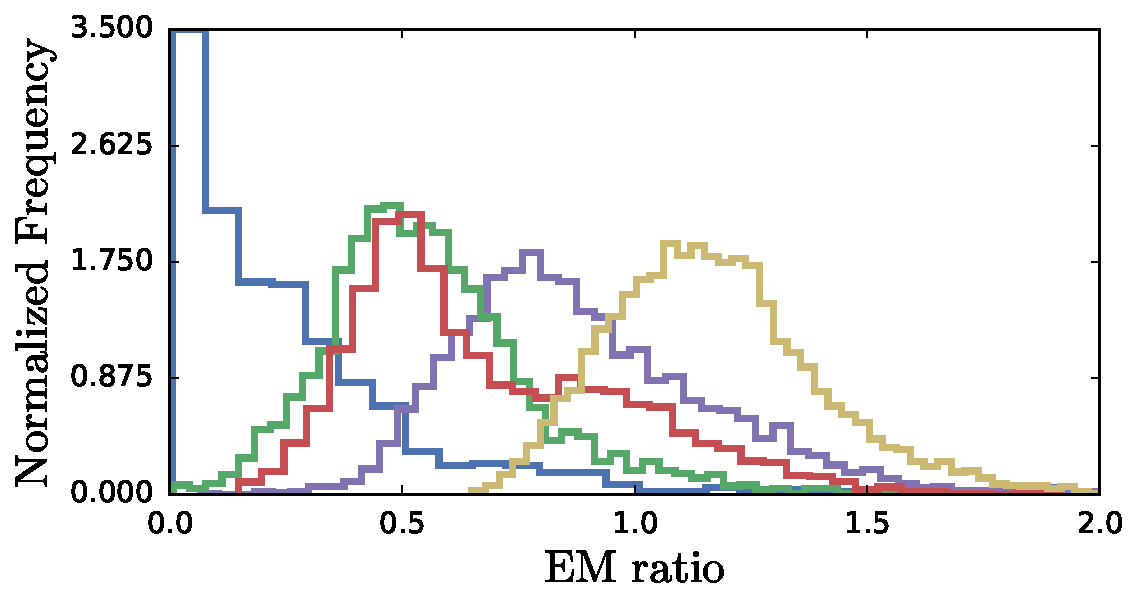
\includegraphics[width=0.49\columnwidth]{figures/ratio_hist_twait_ion_T2.pdf}
        \label{fig:ratio_ion_twait}}
        \caption{Histograms of emission measure ratios for the entire multidimensional heating parameter space (see Fig. \ref{fig:parameter_space}). Each histogram is normalized such that for each distribution $P(x)$, $\int^{\infty}_{-\infty}\mathrm{d}x\,P(x)=1$ and the bin widths are calculated using the well-known Freedman-Diaconis formula \citep{freedman_histogram_1981}. The top panels show the electron heating cases and the bottom panels show the ion heating cases. In the left panels, each histogram (denoted by linestyle and color) corresponds to a unique heating function $(\alpha,\beta)$. The uniform case has not been included here. In the right panels, the emission measure ratios are grouped by $t_N$. Here we show only five values of $t_N$ for aesthetic reasons.}
      \end{figure}
      \vspace{-2ex}
    \end{block}
    %conclusions
    \begin{block}{Conclusions}
      \vspace{-1ex}
      \begin{itemize}
        \item While cool part of $\mathrm{EM}(T)$ more elongated for $\beta=1$, \alert{hot part of emission measure distribution independent of $\beta$}.
        \item For intermediate heating frequencies, power-law cases (compared to uniform case) show significantly more hot emission, for both electron and ion heating
        \item Compared to single-nanoflare results, ion heating results show $\mathrm{EM}(T)$ extending to hotter temperatures ($>10^7$ K) for intermediate to low heating frequencies
        \item \alert{Effects due to NEI only important for uniform heating in electron heating case}, no visible differences in ion heating case
        \item Emission measure ratio seems to be largely independent of $\alpha$, weakly dependent on $\beta$.
        \item \alert{In ion heating case, lower $t_N$ required for consistency with \citet{brosius_pervasive_2014} results as compared to electron heating case}.
      \end{itemize}
      \vspace{-1ex}
    \end{block}
    %references
    \begin{block}{References}
      \scriptsize
      \vspace{-2ex}
      \begin{multicols}{2}
        \bibliographystyle{apj}
        \bibliography{astrophys-abbrev.bib,references.bib}
      \end{multicols}
      This work was supported in part by the Big-Data Private-Cloud Research Cyberinfrastructure MRI-award funded by NSF under grant CNS-1338099 and by Rice University.
    \end{block}
  \end{column}
  \end{columns}
\end{frame}
\end{document}
